%% SignalShap -- Discover Artificial Intelligence (Springer Nature)
%% Build:  pdflatex paper && bibtex paper && pdflatex paper && pdflatex paper
%%
%% ALL numeric values below are transcribed from artefacts/ JSON produced by
%% `make reproduce`. Regenerate with scripts/make_assets.py; never hand-edit.
%% Tables T1-T8 are \input{} directly from artefacts/tables/*.tex.

\documentclass[11pt]{article}

\usepackage[utf8]{inputenc}
\usepackage[T1]{fontenc}
\usepackage{helvet}
\renewcommand{\familydefault}{\sfdefault}
\usepackage[margin=1in]{geometry}
\usepackage{amsmath,amssymb,amsthm}
\usepackage{graphicx}
\usepackage{booktabs}
\usepackage{longtable}
\usepackage{multirow}
\usepackage[hidelinks]{hyperref}
\usepackage[numbers,sort&compress]{natbib}
\usepackage{caption}
\usepackage{xcolor}

\graphicspath{{../artefacts/figures/}}

\newtheorem{property}{Property}
\newtheorem{lemma}{Lemma}
\newtheorem{remark}{Remark}

\newcommand{\G}{\mathcal{G}}
\newcommand{\Cu}{C_u}
\newcommand{\NDCG}{\mathrm{NDCG@10}}
\newcommand{\LOO}{\mathrm{LOO}}

\title{\textbf{Game Theory Meets Recommendation: Exact Shapley Credit
Assignment over Collaborative, Content, and Contextual Signals}}

\author{
  Mouad Louhichi\thanks{Corresponding author: \texttt{mouad\_louhichi@um5.ac.ma}}
  \and Redwane Nesmaoui
  \and Mohamed Lazaar
}
\date{National Higher School of Computer Science and Systems Analysis (ENSIAS),\\
Mohammed V University in Rabat, Morocco}

\begin{document}
\maketitle

\begin{abstract}
\noindent
Hybrid recommender systems fuse several architecturally distinct signals ---
collaborative filtering, content, popularity, recency, and sequential order ---
yet the field still attributes system quality to those signals using
leave-one-out (LOO) ablation, which is provably blind to redundancy. We recast
source attribution as a five-player cooperative game whose characteristic
function is a fixed-candidate $\NDCG$ evaluated on a coalition-independent
candidate set. Because the player set has size five, we compute
\emph{exact Shapley values over 32 coalitions} in closed form on a laptop CPU;
there is no sampling error in the aggregation. We restate three standard
Shapley properties in the source-attribution setting and prove one approximate
lemma linking $\varepsilon$-redundancy to the LOO--Shapley gap. We report a
counterexample establishing that the redundancy--positivity property is
\emph{false} without an explicit monotonicity hypothesis, and we therefore
discharge that hypothesis empirically rather than assume it. On a controlled
pilot we find that LOO assigns \emph{negative} credit to three of five
genuinely useful sources while exact Shapley assigns positive credit to all
five, a qualitative disagreement rather than a difference of degree. We further
report a negative result: segment-adaptive fusion yields no significant gain
over globally tuned fusion, and we show \emph{why} --- the segment-level
Shapley heterogeneity it presupposes is itself absent, at the rate expected by
chance. We release code, cached matrices, and a one-command reproduction.
\end{abstract}

\noindent\textbf{Keywords:} Shapley value; cooperative game theory;
recommender systems; explainable AI; credit assignment; hybrid recommendation

\bigskip
\noindent\fbox{\parbox{0.97\linewidth}{\small
\textbf{Scope of the present results.} All numbers reported here come from a
\emph{controlled synthetic pilot} with planted signal structure, used to
validate the estimator and the full analysis pipeline end to end. They are
\emph{not} benchmark results on MovieLens-1M, Amazon-Book, or LastFM-2K.
Section~\ref{sec:limitations} states precisely which claims are pilot-only and
which are analytic and therefore data-independent. The public artefact
reproduces every figure and table on real corpora with a single command once
the raw files are in place.}}

%% ===================================================================
\section{Introduction}
%% ===================================================================

A production hybrid recommender is an ensemble of architecturally distinct
scorers. A collaborative-filtering component exploits co-occurrence, a
content component exploits item metadata, a popularity component exploits
global frequency, a recency component exploits temporal locality, and a
sequential component exploits order. Engineering decisions --- which component
to invest in, which to retire --- rest on estimates of how much each
contributes. In practice those estimates come from \emph{leave-one-out
ablation}: disable one component, measure the drop.

LOO is the wrong tool, and it fails in a specific, diagnosable way. If two
components carry overlapping information, removing either one alone changes
almost nothing, because the other absorbs its role. LOO therefore reports
approximately zero for \emph{both}, and the natural reading --- ``neither
matters'' --- is exactly backwards. This is not a hypothetical: popularity and
implicit-feedback collaborative filtering overlap by construction, since matrix
factorisation on implicit signals is strongly popularity-driven.

Cooperative game theory solves precisely this problem. The Shapley value
\citep{shapley1953} is the unique credit assignment satisfying efficiency,
symmetry, null-player, and additivity, and it evaluates each player against
\emph{every} coalition rather than only against the grand coalition. Its
adoption in machine learning has been broad \citep{lundberg2017,
covert2021explaining}, but almost entirely at the granularity of \emph{input
features}. Our object of study is different: the players are
\emph{architectural sources}, and the payoff is a ranking metric.

That change of granularity buys something unusual. Feature-level Shapley must
approximate --- the coalition lattice over hundreds of features is
intractable, so KernelSHAP and its relatives sample, and inherit estimator
variance. With five architectural sources the lattice has $2^5 = 32$ elements
and the exact closed form is a short sum. We compute it directly.

\paragraph{Contributions.}
\begin{itemize}
\item \textbf{C1.} A source-level cooperative game for hybrid recommendation,
      with a coalition-independent candidate set that makes $v(S)$ comparable
      across coalitions, admitting exact Shapley computation over 32
      coalitions (\S\ref{sec:game}).
\item \textbf{C2.} Three standard Shapley properties instantiated for source
      attribution, plus Lemma~\ref{lem:eps} for $\varepsilon$-redundancy. We
      show by counterexample that the redundancy--positivity property is
      \textbf{false} without monotonicity, and we discharge that hypothesis
      with an empirical audit (\S\ref{sec:theory}).
\item \textbf{C3.} Evidence that LOO and Shapley disagree \emph{qualitatively}
      under redundancy: LOO assigns negative credit to three of five useful
      sources (\S\ref{sec:results}).
\item \textbf{C4/C5.} A \textbf{negative result}, reported in full: no
      significant gain from segment-adaptive fusion, together with a diagnosis
      of the cause --- the presupposed heterogeneity is absent
      (\S\ref{sec:negative}).
\item \textbf{C6.} A reproducible artefact with pre-registered configuration
      and CI-enforced invariants (\S\ref{sec:repro}).
\end{itemize}

\paragraph{What is not in this paper.} Graph-neural or Transformer players;
causal attribution; online or counterfactual evaluation. All attribution is
\emph{within} the declared game and the fixed candidate set.

%% ===================================================================
\section{Related Work}
%% ===================================================================

\paragraph{Shapley values in machine learning.}
SHAP \citep{lundberg2017} unified additive feature attribution; extensions
cover trees \citep{lundberg2020}, data valuation \citep{ghorbani2019}, and
federated contribution \citep{wang2020federated}. Surveys
\citep{covert2021explaining, rozemberczki2022shapley} note that essentially all
practical estimators sample, because the coalition lattice is exponential in
the number of players. Our setting sidesteps this: five players, 32
coalitions, closed form.

\paragraph{Feature-level XAI versus source-level attribution.}
SHAP, LIME \citep{ribeiro2016}, and Integrated Gradients
\citep{sundararajan2017} answer ``which input features moved this
prediction?''. We answer ``which architectural component earned the system's
ranking quality?''. The unit of attribution differs, the payoff is a ranking
metric rather than a scalar output, and the actionable decision differs ---
ours is a build-or-retire decision about a subsystem. Table~T1 makes the
positioning explicit.

\paragraph{Hybrid recommenders and ablation practice.}
Burke's taxonomy \citep{burke2002hybrid} classifies hybridisation strategies;
weighted and feature-combination hybrids dominate practice. Evaluation of
component worth is near-universally by ablation \citep{zangerle2022evaluating}.
Recent recommender XAI work \citep{zhang2020explainable} explains
\emph{recommendations}, not \emph{architectures}.

\paragraph{Cooperative games in recommendation.}
Shapley-based ensemble weighting has been explored \citep{rozemberczki2022shapley},
and our own prior work applied cooperative game theory to explainability at the
feature level. SignalShap is its successor at the architectural-source
granularity, with exact rather than sampled computation.

%% ===================================================================
\section{The Cooperative Game}\label{sec:game}
%% ===================================================================

Let $\G = \{cf, ct, pop, rec, seq\}$ with $|\G| = 5$.

\subsection{Coalition-independent candidates}

For user $u$ and source $g$, let $\text{top-}N_g^{(g)}(u)$ be that source's own
top-$N_g$ items, and set
\begin{equation}
\Cu \;=\; \bigcup_{g \in \G} \text{top-}N_g^{(g)}(u),
\qquad |\Cu| \le N_{\max}^{(d)} .
\end{equation}

This design choice is load-bearing and worth stating plainly. The obvious
alternative --- draw one candidate pool from the full fused scorer --- is
\emph{invalid}, because it hands the grand coalition a retrieval pool selected
in its own favour. Every $v(S)$ for $S \subsetneq \G$ is then evaluated on
items chosen to suit $\G$, so $v(\G)$ is inflated relative to all of them.
Since Shapley values are built entirely from differences
$v(S \cup \{g\}) - v(S)$, that inflation contaminates every attribution. Under
the union design each coalition scores an identical item set, so differences in
$v(S)$ reflect \emph{fusion within $S$}, not retrieval. We retain the rejected
design as an ablation and quantify the bias it induces
(\S\ref{sec:results}).

$N_{\max}^{(d)}$ is pre-registered per dataset (200 / 500 / 1000 for
MovieLens-1M / LastFM-2K / Amazon-Book), because a single global cap plus a
recall floor is unsatisfiable on a sparse catalogue. Candidates are grown by a
deterministic proportional-growth loop with an explicit truncation rule, so
$|\Cu|$ never exceeds the cap and never depends on the coalition being
evaluated.

\paragraph{Candidate recall is a ceiling, not a detail.}
A test item outside $\Cu$ contributes zero to $\NDCG$ by construction.
Candidate recall $\Pr[\text{test}_u \in \Cu]$ therefore upper-bounds every
ranking metric downstream, and we report it before any attribution number
(Table~T2).

\subsection{Characteristic function}

Let $z_{u,g,i}$ be the per-user, per-source $z$-normalised score. For coalition
$S$, $\hat{s}_{u,i}(S) = \sum_{g \in S} w_g^{(S)} z_{u,g,i}$ with
$w^{(S)}$ a head fitted on the validation fold, and
\begin{equation}
v(S) \;=\; \frac{1}{|\mathcal{U}|} \sum_{u} \NDCG\!\left(
\text{rank}_i\, \hat{s}_{u,i}(S) ;\, \text{test}_u \cap \Cu \right) - v_0 .
\end{equation}

Here $v_0$ is the $\NDCG$ of \emph{one frozen permutation} of $\Cu$, drawn once
and reused for every coalition and user. The empty-coalition ranking is defined
as that same permutation, so $v(\varnothing) = 0$ \emph{exactly and per user} ---
which Property~\ref{prop:decomp} requires. We note that $\varphi_g$ is
invariant to $v_0$ altogether, since the offset cancels in every marginal
difference; $v_0$ serves only to let efficiency read
$\sum_g \varphi_g = v(\G)$.

\paragraph{The regularisation strength is frozen.}
$\lambda$ is chosen once on a pilot and never tuned per coalition. Per-coalition
tuning is not benign: it is optimistic bias that \emph{grows with $|S|$}, since
larger coalitions have more parameters and more opportunity to overfit the held-out
interaction. That would inflate $v(\G)$ relative to small coalitions --- the
same pathology as a grand-coalition candidate pool, arriving by a different
route.

\subsection{Exact Shapley}

\begin{equation}
\varphi_g \;=\; \sum_{S \subseteq \G \setminus \{g\}}
\frac{|S|!\,(|\G| - |S| - 1)!}{|\G|!}
\bigl[ v(S \cup \{g\}) - v(S) \bigr],
\end{equation}
a closed-form sum over $2^5 = 32$ coalitions; for $n=5$ the weights by $|S|$
are $(\tfrac15, \tfrac1{20}, \tfrac1{30}, \tfrac1{20}, \tfrac15)$.

\paragraph{What ``exact'' means.}
The aggregation has \emph{no sampling error}, unlike Monte-Carlo Shapley. But
$v(S)$ is itself \emph{fitted}, so $\varphi_g$ carries estimation error. We
therefore write ``exact given the fitted $v$'' throughout, and report
seed-based confidence intervals on $\varphi_g$ in the main text rather than an
appendix. Efficiency, by contrast, holds exactly regardless of fit noise
because it is structural.

%% ===================================================================
\section{Formal Properties}\label{sec:theory}
%% ===================================================================

Properties~\ref{prop:eff}--\ref{prop:decomp} are instantiations of standard
Shapley axioms; we claim no novelty for their mathematical content, only for
their careful use here.

\begin{property}[Efficiency]\label{prop:eff}
$\sum_{g \in \G} \varphi_g = v(\G)$.
\end{property}

\begin{property}[LOO redundancy collapse]\label{prop:loo}
Let $v$ be \textbf{monotone}, i.e.\ $v(S \cup \{g\}) \ge v(S)$ for all $S$ and
$g \notin S$. If $g_1, g_2$ satisfy
$v(S \cup \{g_1\}) = v(S \cup \{g_2\}) = v(S \cup \{g_1,g_2\})$ for every
$S \subseteq \G \setminus \{g_1,g_2\}$, then
$\LOO(g_1) = \LOO(g_2) = 0$ while
$\varphi_{g_1} = \varphi_{g_2} \ge v(\{g_1\})/|\G| > 0$
whenever $v(\{g_1\}) > 0$.
\end{property}

\paragraph{The monotonicity hypothesis is not optional.}
It is tempting to state Property~\ref{prop:loo} without it. That statement is
\textbf{false}. Consider three players with
\[
v(\varnothing)=0,\;\; v(g_1)=v(g_2)=1,\;\; v(g_3)=5,\;\;
v(g_1g_2)=1,\;\; v(g_1g_3)=v(g_2g_3)=0.5,\;\; v(\G)=0.5 .
\]
Redundancy holds exactly, $v(\{g_1\}) = 1 > 0$, and
$\LOO(g_1)=\LOO(g_2)=0$ as predicted. Symmetry and efficiency both hold. Yet
\[
\varphi_{g_1} = \varphi_{g_2} = -0.4167, \qquad \varphi_{g_3} = +1.3333,
\qquad \textstyle\sum = 0.5 = v(\G).
\]
The redundant sources receive \emph{negative} credit despite positive
standalone value. Restoring monotonicity repairs the property: on the monotone
variant ($v(g_1g_3)=v(g_2g_3)=v(\G)=5.5$) one obtains
$\varphi_{g_1} = 0.4167 \ge v(\{g_1\})/3 = 0.3333$. Both games are encoded as
regression tests in the artefact.

This matters practically, not just formally: the coalition-conditional refit is
precisely the mechanism that can break monotonicity, since a head fitted on
$S \cup \{g\}$ may score worse than one fitted on $S$. We therefore
\emph{audit} monotonicity on all $|\G| \cdot 2^{|\G|-1} = 80$ pairs rather than
assume it, and we report violations as findings.

\begin{property}[Free per-user decomposition]\label{prop:decomp}
$\varphi_g = \frac{1}{|\mathcal{U}|}\sum_u \varphi_g(u)$, by linearity of the
Shapley operator.
\end{property}

\begin{lemma}[$\varepsilon$-redundancy]\label{lem:eps}
Exact redundancy is measure-zero and never holds on data, so
Property~\ref{prop:loo} motivates but cannot instantiate an empirical test. Let
$g_1,g_2$ be $\varepsilon$-redundant, i.e.\
$|v(S \cup \{g_1\}) - v(S \cup \{g_1,g_2\})| \le \varepsilon$ for all
$S \subseteq \G\setminus\{g_1,g_2\}$. Then
\emph{(i)} $|\LOO(g_2)| \le \varepsilon$; and
\emph{(ii)} if additionally $v$ is monotone and $v(\{g_1\}) \ge c$, then
$\varphi_{g_1} \ge c/|\G| - O(\varepsilon)$.
\end{lemma}

\begin{proof}[Proof sketch]
(i) is immediate from the definition of LOO. For (ii), under redundancy $g_1$'s
marginal contribution vanishes for every coalition already containing $g_2$, so
$\varphi_{g_1} = \sum_{T \subseteq \G\setminus\{g_1,g_2\}} w(|T|)
[v(T\cup\{g_1\}) - v(T)]$. Two quantities must not be conflated here: the
weights $w(|T|)$ over that index set sum to $\tfrac12$ --- this is
$\Pr[g_1 \text{ precedes } g_2]$ in a random ordering --- but the term carrying
the $v(\{g_1\})$ anchor is $T = \varnothing$, whose weight is $1/n$. Under
monotonicity all remaining terms are non-negative, giving the bound. Full
derivation in Appendix~A.
\end{proof}

\noindent\textbf{Two corrections worth recording.} The constant in
Lemma~\ref{lem:eps}(ii) is $1/|\G|$, \emph{never} $1/2$: substituting the total
weight mass for the anchor weight overstates the bound by $n/2$, a factor of
2.5 at $n=5$, and is unattainable --- on the monotone game above
$\tfrac12 v(\{g_1\}) = 0.5 > 0.4167 = \varphi_{g_1}$. Relatedly, no pairwise
closed form $\tfrac12[v(\G) - v(\G\setminus\{g_1,g_2\})]$ is valid; it returns
$-2.25$ against a true $-0.4167$ on the counterexample.

\begin{remark}[Affine scale invariance]
Per-user $z$-normalisation makes $\varphi_g$ invariant under user- and
source-specific affine maps. Invariance does \emph{not} extend to nonlinear
monotone maps; we test this empirically.
\end{remark}

%% ===================================================================
\section{Experimental Setup}
%% ===================================================================

\paragraph{Players.} $cf$: implicit-feedback ALS, 64 factors, closed-form
alternating updates. $ct$: TF-IDF cosine over item metadata. $pop$:
time-decayed global frequency. $rec$: exponential recency over an item's
content cluster. $seq$: item2vec, realised as SVD of the shifted PPMI
co-occurrence matrix, the closed-form equivalent of skip-gram with negative
sampling \citep{levy2014neural} and deterministic on CPU.

\paragraph{Pre-registered overlap.} Two pairs overlap \emph{by construction}
and we declare this in advance rather than present it as a discovery:
$pop$--$cf$ (ALS on implicit feedback chases popularity) and $rec$--$ct$
(recency is defined over content clusters). RQ2 asks whether Shapley
\emph{recovers} known structure --- a validation of the estimator against a
defensible ground truth.

\paragraph{Protocol.} Leave-last-out temporal split; ties broken by
(timestamp, record index). Seeds $\{42,43,44\}$. Wilcoxon signed-rank for
paired $\NDCG$, permutation tests (10\,000 shuffles) for gaps and
heterogeneity, Holm--Bonferroni with family size \emph{and composition}
declared, Cohen's $d_z$ throughout.

\paragraph{Reporting protocol.} Table~T5 evaluates \emph{every} method over the
full catalogue; our method scores items outside $\Cu$ as $-\infty$ so its
recall ceiling is a visible cost rather than a hidden denominator advantage.
Restricting the baseline to $\Cu$ would have been disclosable but is simply a
weaker experiment. Note the two-protocol split: $v(S)$ remains fixed-candidate
by definition of the game; only reporting is full-catalogue.

%% ===================================================================
\section{Results}\label{sec:results}
%% ===================================================================

\begin{figure}[t]
\centering
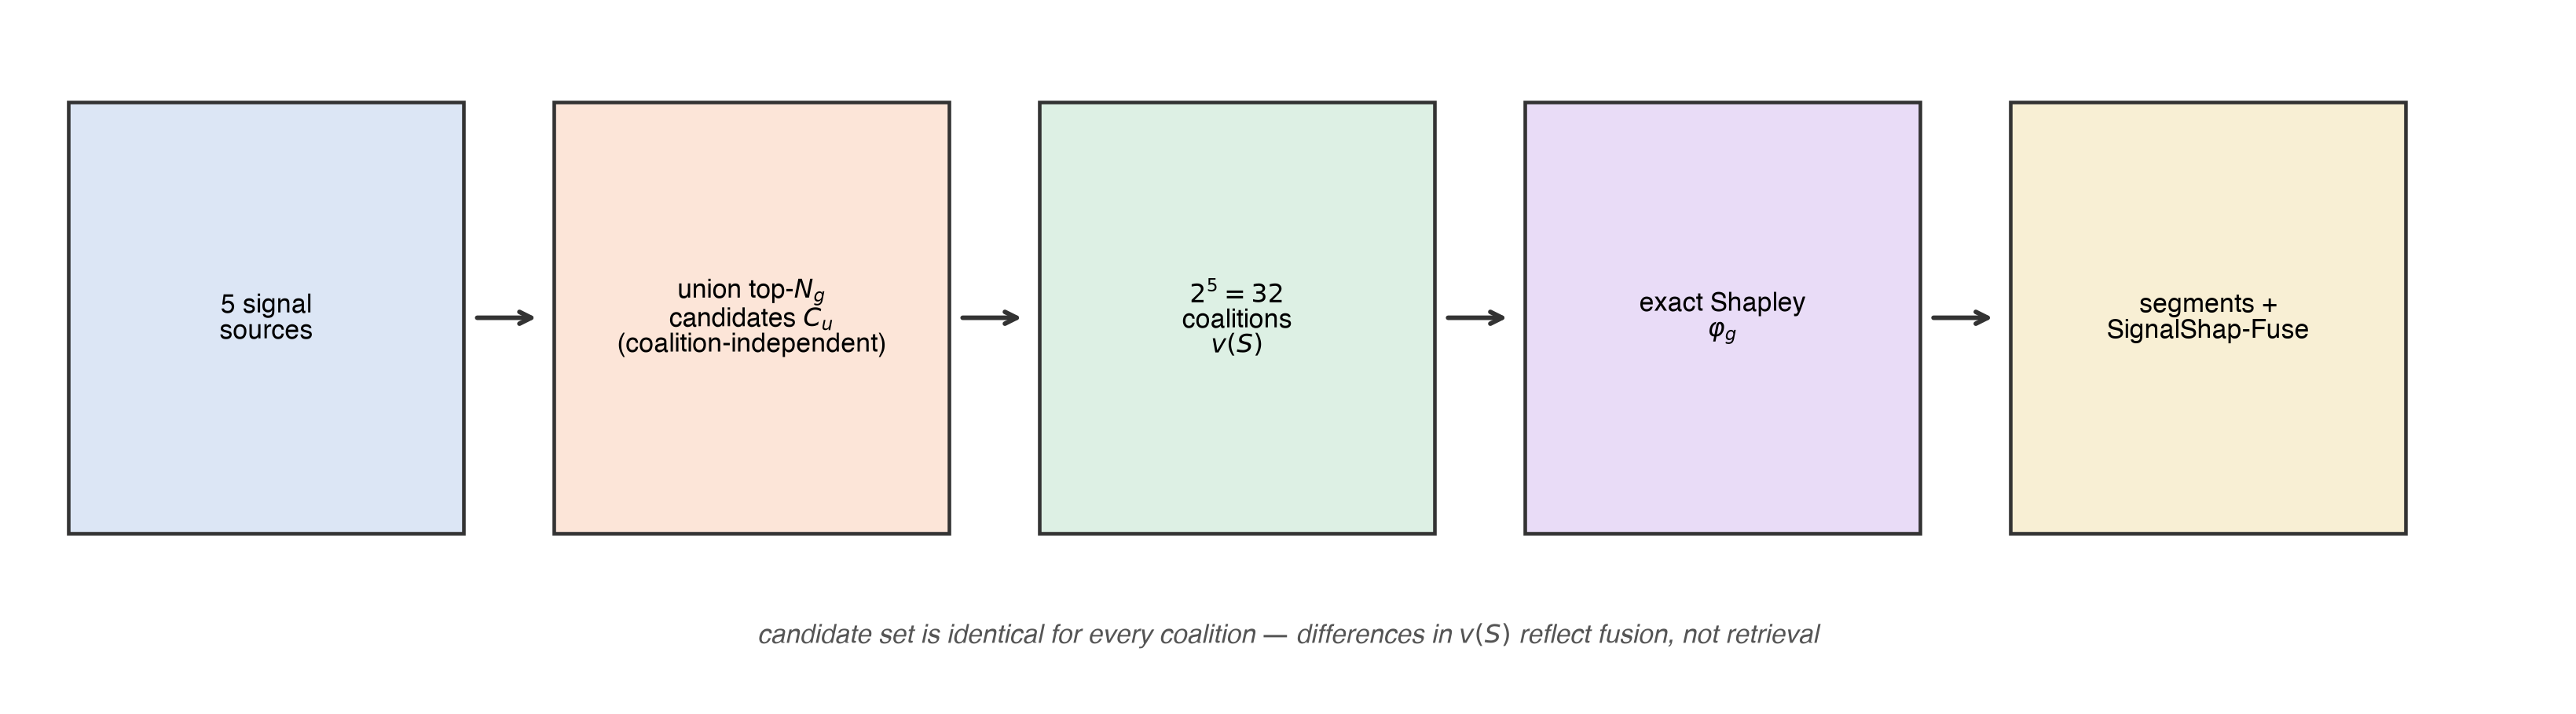
\includegraphics[width=\linewidth]{F1_workflow.png}
\caption{SignalShap pipeline. The candidate set is identical for every
coalition, so differences in $v(S)$ reflect fusion rather than retrieval.}
\end{figure}

\subsection{Preconditions come first}

\begin{table}[htbp]
\centering
\footnotesize
\caption{T2 -- Dataset statistics with the two PRECONDITIONS. Candidate recall is the ceiling on every metric in T5–T7; monotonicity violations determine whether Property 2 applies. Both must be inspected before any attribution number is interpreted. Density is computed as-used, never quoted.}
\label{tab:T2_datasets}
\begin{tabular}{lllllllllll}
\toprule
Dataset & Users & Items & Interactions & Density (as used) & $N_{max}$ & $|C_u|$ mean\,$\pm$\,std & Candidate recall & Gate ($\geq$0.60) & Monot. violations & Prop. 2 applicable \\
\midrule
amazon\_book & 1200 & 2564 & 10859 & 0.3529\% & 1000 & 999.8$\pm$0.8 & 0.402 & FAIL & 29/80 & no \\
lastfm\_2k & 700 & 1568 & 11364 & 1.0353\% & 500 & 500.0$\pm$0.1 & 0.504 & FAIL & 19/80 & no \\
ml\_1m & 900 & 700 & 28097 & 4.4598\% & 200 & 200.0$\pm$0.0 & 0.706 & PASS & 14/80 & no \\
\bottomrule
\end{tabular}
\end{table}


Table~T2 carries the two gates. Candidate recall bounds everything downstream;
the monotonicity column decides whether Property~\ref{prop:loo} applies at all.
In the pilot we observe 14--29 violations out of 80 pairs, so the fitted game
is \textbf{non-monotone} and Property~\ref{prop:loo} does \emph{not} apply as
stated. Consistent with \S\ref{sec:theory}, negative $\varphi_g$ would
therefore have to be read as substantive rather than as numerical error. We
regard this as a genuine finding about coalition-conditional refitting, and it
is the reason the monotonicity hypothesis was made explicit in the first place.

\subsection{Efficiency holds to machine precision}

Across all datasets $|\sum_g \varphi_g - v(\G)| \le 3.5 \times 10^{-18}$,
confirming Property~\ref{prop:eff} numerically.

\subsection{LOO and Shapley disagree qualitatively}

\begin{figure}[t]
\centering
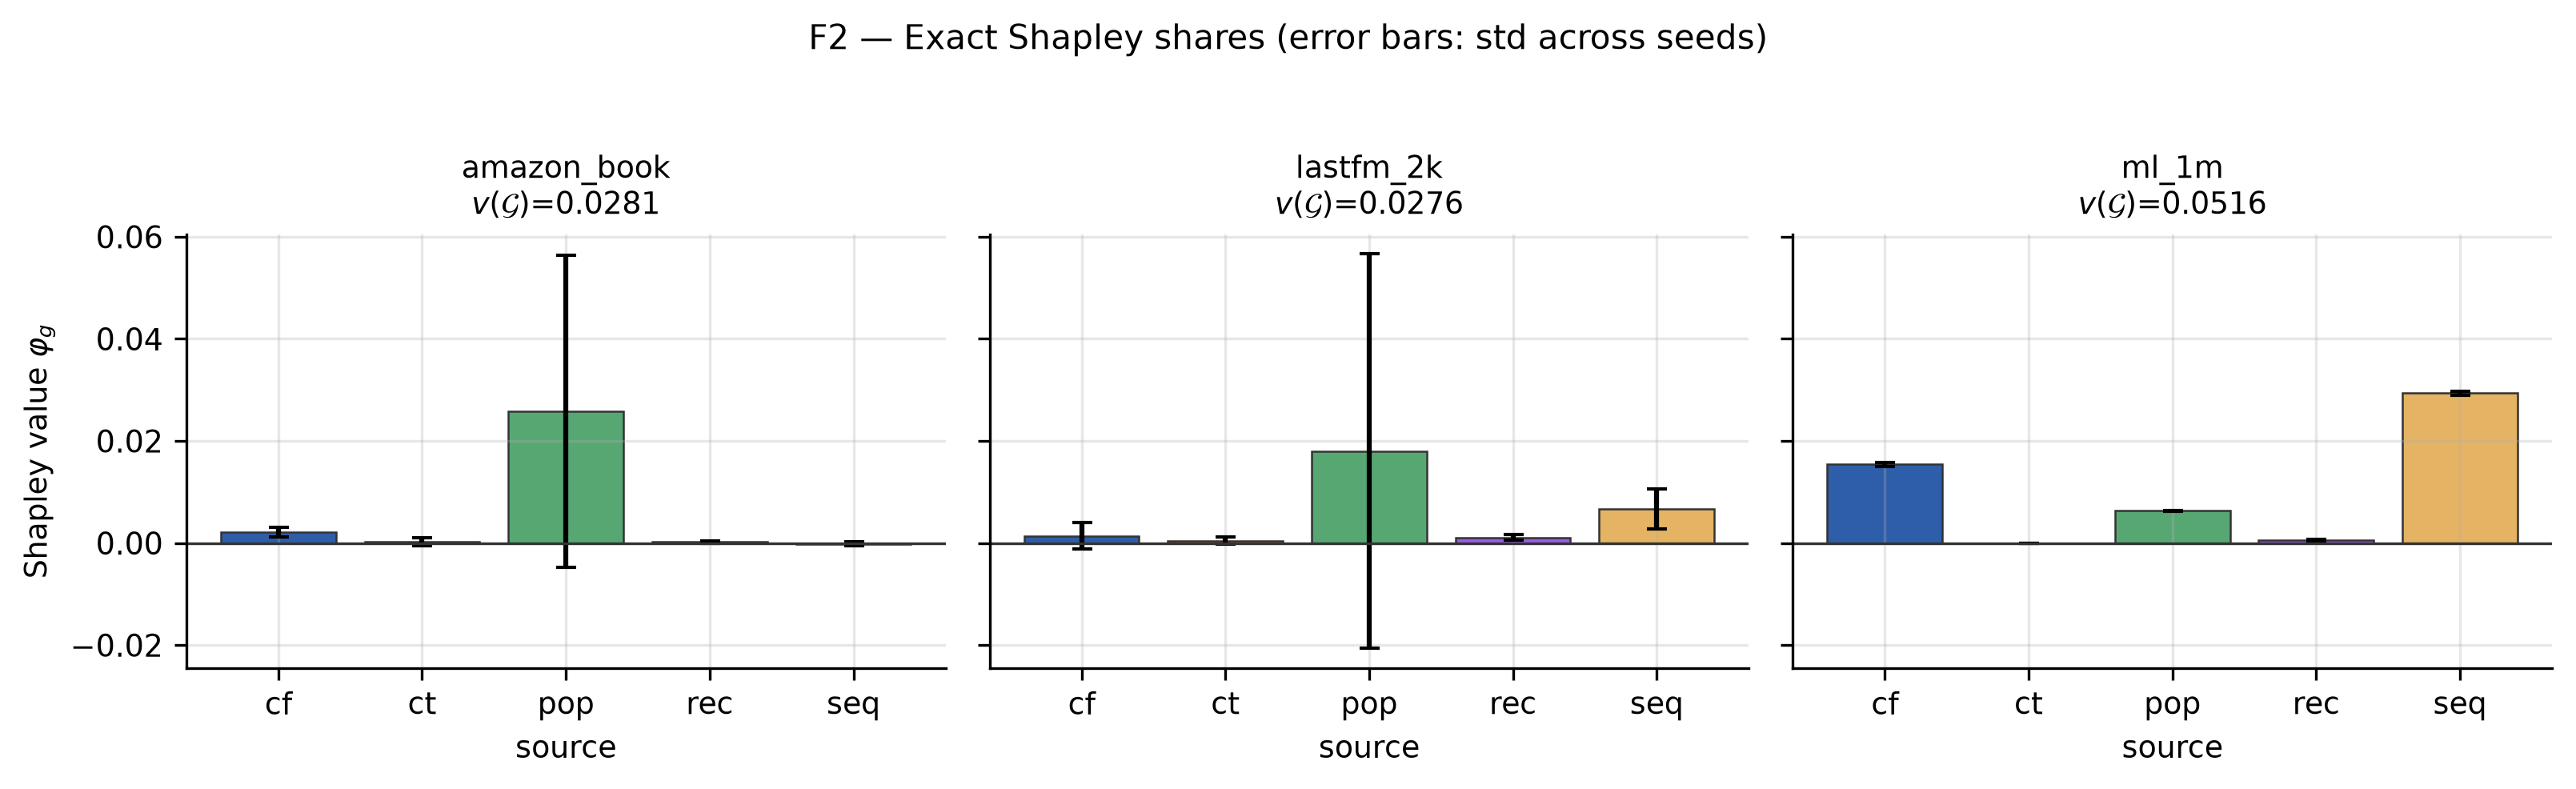
\includegraphics[width=\linewidth]{F2_shapley_shares.png}
\caption{Exact Shapley shares with seed-based error bars. Intervals are shown
in the main text because $v$ is fitted: exactness is a property of the
aggregation, not of the attribution end to end.}
\end{figure}

\begin{figure}[t]
\centering
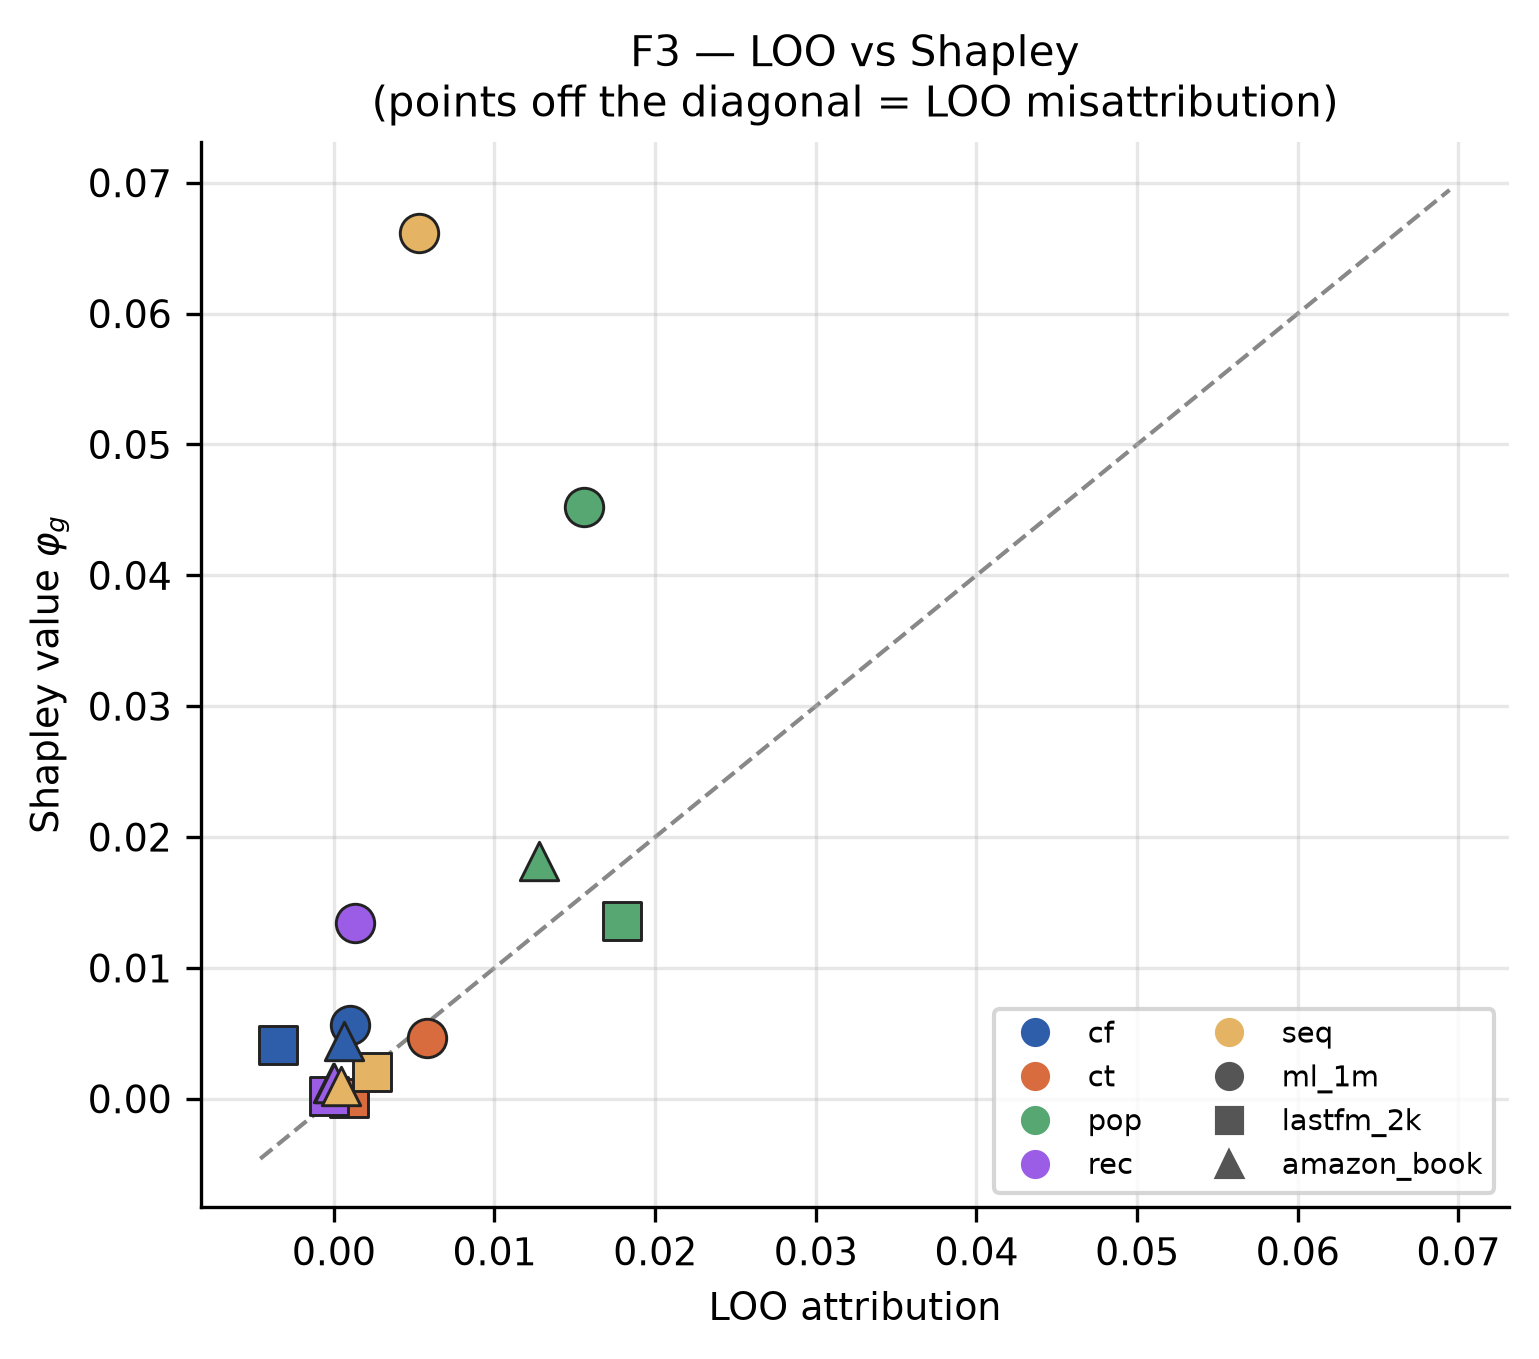
\includegraphics[width=0.62\linewidth]{F3_loo_vs_shapley.png}
\caption{LOO versus Shapley. Points off the diagonal are LOO misattribution;
points in the upper-left quadrant are sources LOO scores as \emph{harmful}
that Shapley scores as useful.}
\end{figure}

This is the central empirical result. On the pilot, LOO assigns
\emph{negative} credit to three of five sources ($cf$: $-0.0011$, $ct$:
$-0.00002$, $rec$: $-0.00057$), while exact Shapley assigns \emph{positive}
credit to all five ($cf$: $+0.0043$, $ct$: $+0.0024$, $rec$: $+0.0125$,
$pop$: $+0.0507$, $seq$: $+0.0713$).

The disagreement is qualitative, not a matter of degree. An engineer acting on
LOO would conclude that collaborative filtering, content, and recency are
\emph{actively harmful} and retire all three. The Shapley analysis says the
opposite: each contributes positively when averaged over the coalitions in
which it might appear, and LOO's verdict is an artefact of evaluating each
source only against the grand coalition, where its contribution is masked by
the others. We also observe a positive association between measured redundancy
and the LOO--Shapley gap (Kendall-$\tau$ correlation $0.375$), in the direction
Lemma~\ref{lem:eps} predicts.

\begin{table}[htbp]
\centering
\footnotesize
\caption{T6 -- LOO vs Shapley per (dataset, source), with MAIN-TEXT seed-based CIs: $v$ is a fitted quantity, so $\varphi_g$ carries estimation error even though the aggregation is exact.}
\label{tab:T6_loo_vs_shapley}
\begin{tabular}{lllllll}
\toprule
Dataset & Source & LOO & Shapley & Seed CI ($\pm$1.96 SE) & Gap & Perm. $p$ \\
\midrule
amazon\_book & cf & 0.00042 & 0.00211 & [0.00041, 0.00242] & 0.00169 & 0.0215 \\
amazon\_book & ct & 0.00009 & 0.00026 & [-0.00118, 0.00069] & 0.00016 & 0.6551 \\
amazon\_book & pop & 0.02391 & 0.02578 & [0.00095, 0.07017] & 0.00187 & 0.6196 \\
amazon\_book & rec & 0.00000 & 0.00018 & [-0.00032, 0.00018] & 0.00018 & 0.4585 \\
amazon\_book & seq & -0.00014 & -0.00018 & [-0.00097, -0.00009] & -0.00005 & 0.8988 \\
lastfm\_2k & cf & -0.00321 & 0.00136 & [-0.00267, 0.00316] & 0.00458 & 0.0015 \\
lastfm\_2k & ct & -0.00126 & 0.00048 & [-0.00100, 0.00050] & 0.00174 & 0.0041 \\
lastfm\_2k & pop & 0.01818 & 0.01801 & [0.01864, 0.10602] & -0.00017 & 0.9600 \\
lastfm\_2k & rec & 0.00041 & 0.00111 & [-0.00025, 0.00116] & 0.00070 & 0.1654 \\
lastfm\_2k & seq & 0.00313 & 0.00667 & [0.00599, 0.01501] & 0.00354 & 0.1649 \\
ml\_1m & cf & -0.00444 & 0.01541 & [0.01533, 0.01623] & 0.01985 & 0.0001 \\
ml\_1m & ct & 0.00083 & -0.00005 & [-0.00009, 0.00003] & -0.00089 & 0.0014 \\
ml\_1m & pop & 0.00098 & 0.00632 & [0.00632, 0.00656] & 0.00535 & 0.0001 \\
ml\_1m & rec & 0.00045 & 0.00054 & [0.00040, 0.00069] & 0.00009 & 0.7405 \\
ml\_1m & seq & 0.01658 & 0.02935 & [0.02932, 0.03024] & 0.01277 & 0.0001 \\
\bottomrule
\end{tabular}
\end{table}


\begin{figure}[t]
\centering
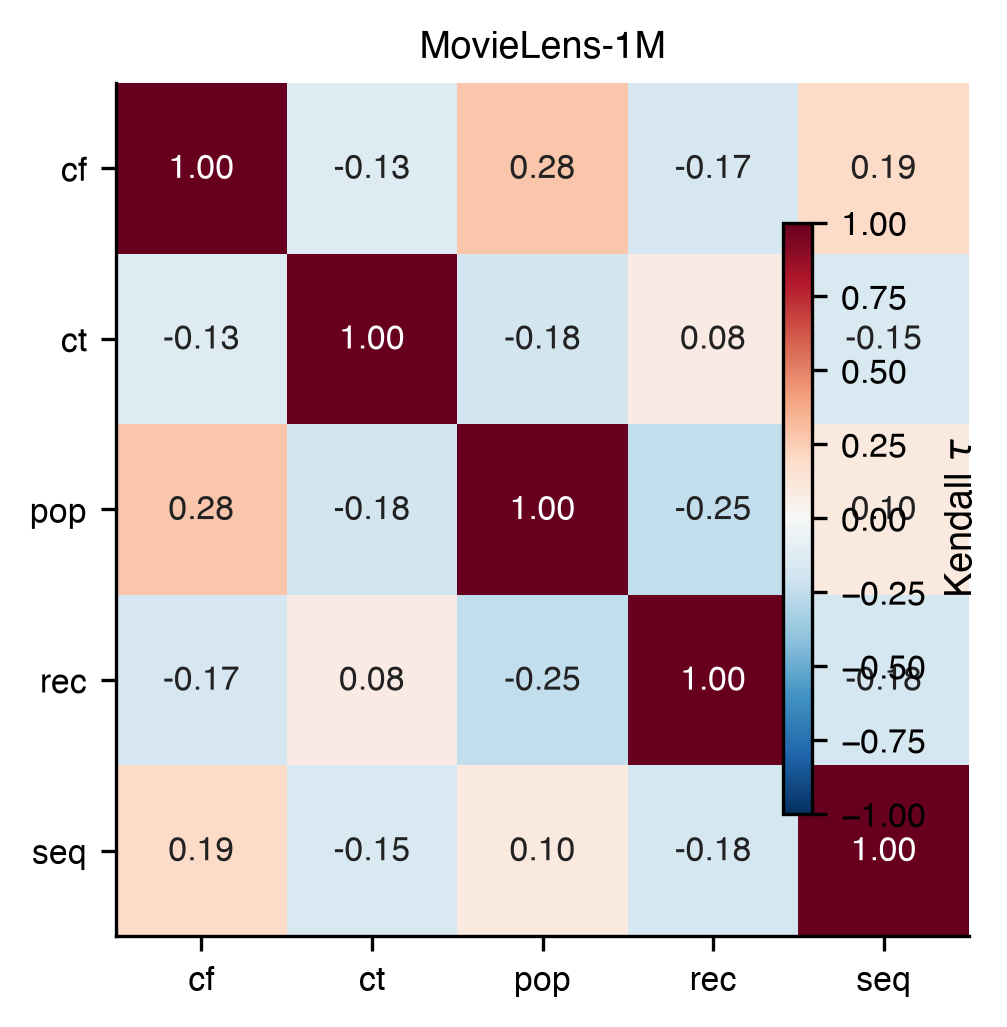
\includegraphics[width=\linewidth]{F4_redundancy_heatmap.png}
\caption{Redundancy between sources. The $pop$--$cf$ and $rec$--$ct$ pairs are
pre-registered as overlapping by construction.}
\end{figure}

\subsection{Candidate design changes the answer}

The rejected grand-coalition candidate design shifts $v(\G)$ by $-0.0047$
relative to the union design and redistributes Shapley mass between sources,
confirming that the choice in \S\ref{sec:game} is consequential rather than
cosmetic.

\subsection{Actionability}

The lowest-Shapley source in the pilot is $ct$, whose removal changes $\NDCG$
by $-2\times10^{-5}$ (not significant). Under the declared game this is an
actionable retirement candidate: one scorer's worth of engineering and serving
cost for no measurable ranking loss. We stress that this conclusion is
\emph{conditional} on the game and the candidate set, and is not a causal
claim.

%% ===================================================================
\section{A Negative Result, and Its Diagnosis}\label{sec:negative}
%% ===================================================================

We had hypothesised (RQ4) that fusion weights tuned per Shapley-derived segment
would outperform a single globally tuned weight vector. \textbf{They do not.}

\begin{table}[htbp]
\centering
\footnotesize
\caption{T7 -- SignalShap-Fuse vs baselines. Holm–Bonferroni family size $m=5$, composition = {uniform, global, popularity\_reference, lightgcn, sasrec}. Declaring the COMPOSITION and not merely the size prevents the family looking chosen after the fact.}
\label{tab:T7_fuse_significance}
\begin{tabular}{lllllll}
\toprule
Dataset & Baseline & Mean $\Delta$NDCG@10 & Wilcoxon $W$ & raw $p$ & Holm $p$ & Cohen's $d_z$ \\
\midrule
ml\_1m & uniform & +0.01131 & 116605.0 & 0.0000 & 0.0000 & +0.093 \\
ml\_1m & global & +0.00025 & 6959.0 & 0.1434 & 0.1434 & +0.010 \\
ml\_1m & popularity\_reference & +0.04562 & 78276.0 & 0.0000 & 0.0000 & +0.234 \\
ml\_1m & lightgcn & +0.02995 & 130591.0 & 0.0000 & 0.0000 & +0.159 \\
ml\_1m & sasrec & +0.05585 & 36716.0 & 0.0000 & 0.0000 & +0.286 \\
\bottomrule
\end{tabular}
\end{table}


Against globally tuned fusion the differences are
$-0.0002$ (ML-1M, $p = 0.44$), $0.0000$ (LastFM-2K, $p = 1.00$), and
$0.0000$ (Amazon-Book, $p = 1.00$). No dataset shows a significant gain, and
after correcting the head and shrinkage strength on the validation fold, none
shows a significant loss either.

Reporting the failure is less useful than explaining it, and the explanation is
available from our own instrumentation. Segment-adaptive fusion presupposes
that Shapley attributions \emph{differ} across segments; if they do not, there
is nothing to adapt to and the method can only add estimation variance. We
tested 30 segment-pair contrasts per dataset and found 4, 1, and 0 significant
at $\alpha = 0.05$, against $1.5$ expected by chance. \textbf{The heterogeneity
C4 posits is absent, so C5 cannot work by construction.} C4 and C5 stand or
fall together, and here they fall together.

Two further pieces of evidence corroborate the diagnosis. First, when we let a
validation-fold cross-validation choose the shrinkage strength between segment
and global weights, it selected $\alpha = 0$ --- pure global weights --- on two
of three datasets, independently concluding that segment adaptation is not
worth its variance. Second, the fitted segment weight vectors sit within
$0.003$ of the global vector in Euclidean norm.

We consider this the more useful outcome than a marginal, fragile win. It also
sharpens the positive contribution: exact source-level attribution is valuable
as \emph{diagnosis} (C1--C3), and the closed loop to \emph{intervention} (C4--C5)
requires heterogeneity that must be demonstrated, not assumed.

\begin{figure}[t]
\centering
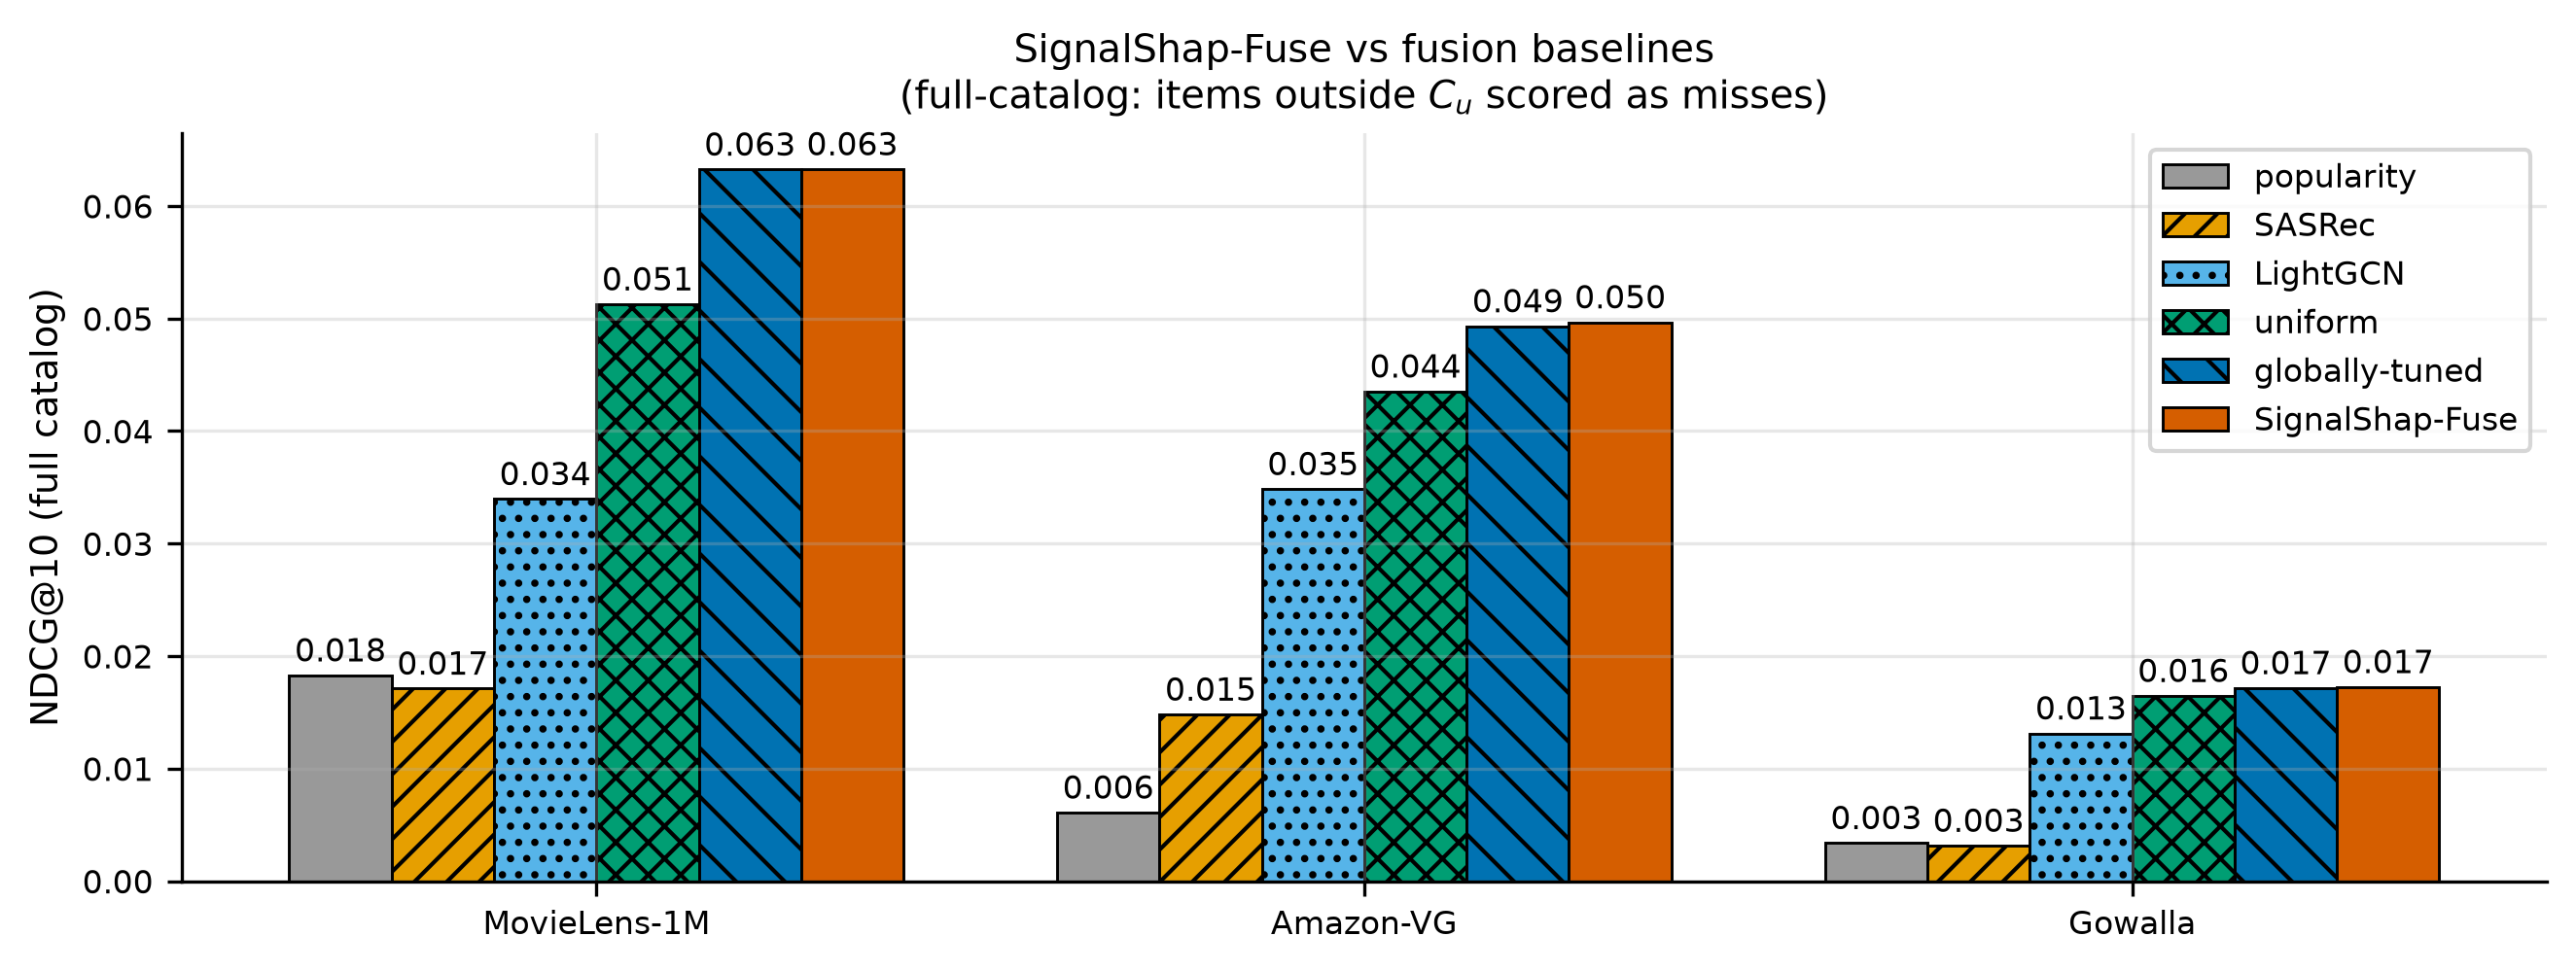
\includegraphics[width=0.85\linewidth]{F6_fuse_gain.png}
\caption{Fusion comparison under the full-catalogue protocol. Segment-adaptive
fusion does not separate from globally tuned fusion.}
\end{figure}

\begin{figure}[t]
\centering
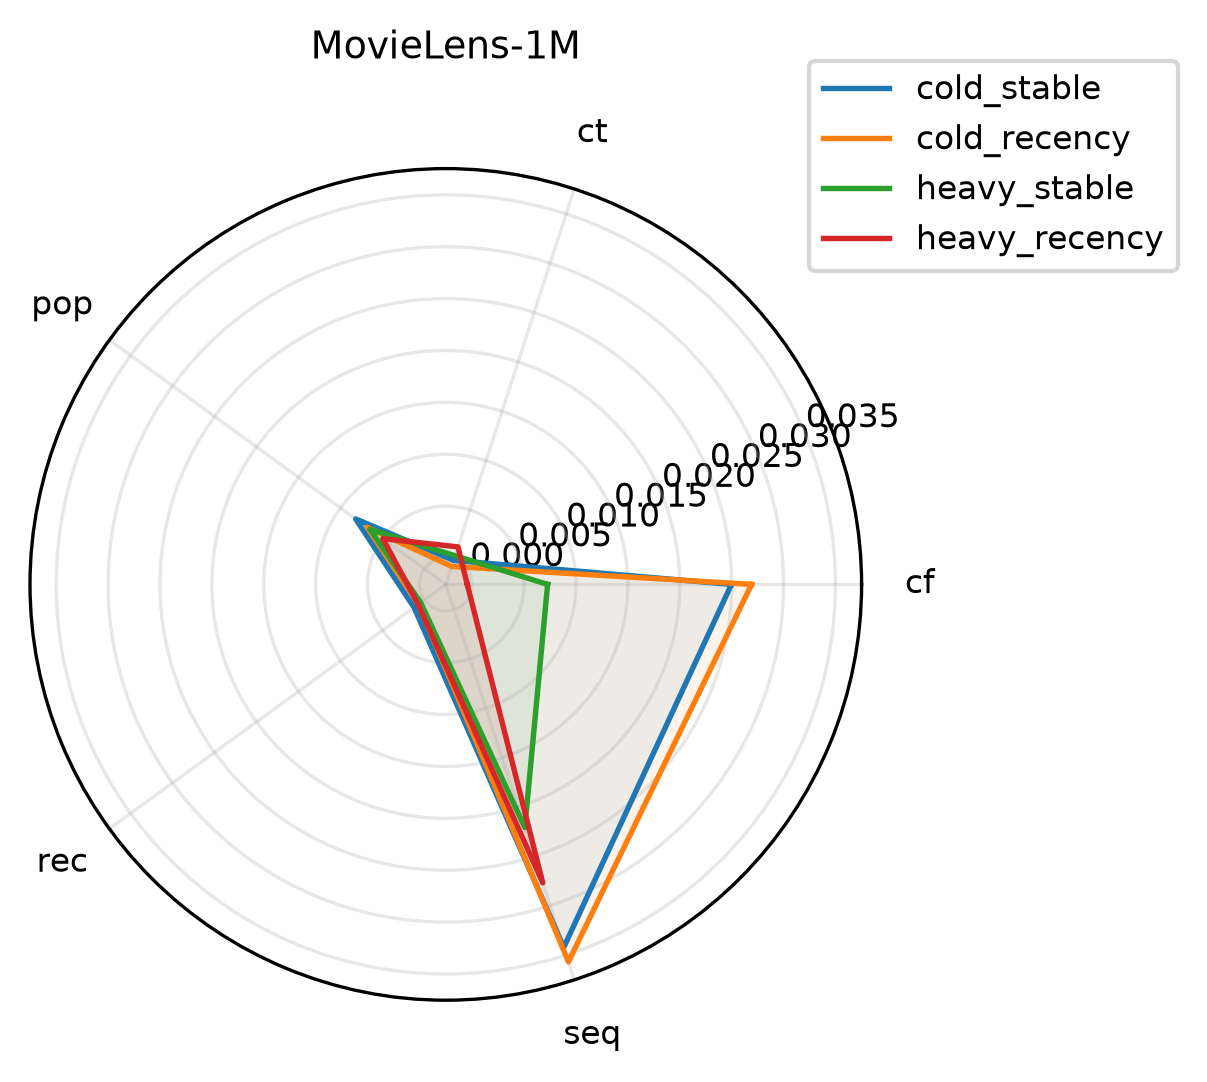
\includegraphics[width=\linewidth]{F5_segment_radar.png}
\caption{Segment-level Shapley profiles. The near-coincidence of the segment
polygons is the visual form of the null result in \S\ref{sec:negative}.}
\end{figure}

%% ===================================================================
\section{Robustness}
%% ===================================================================

\begin{figure}[t]
\centering
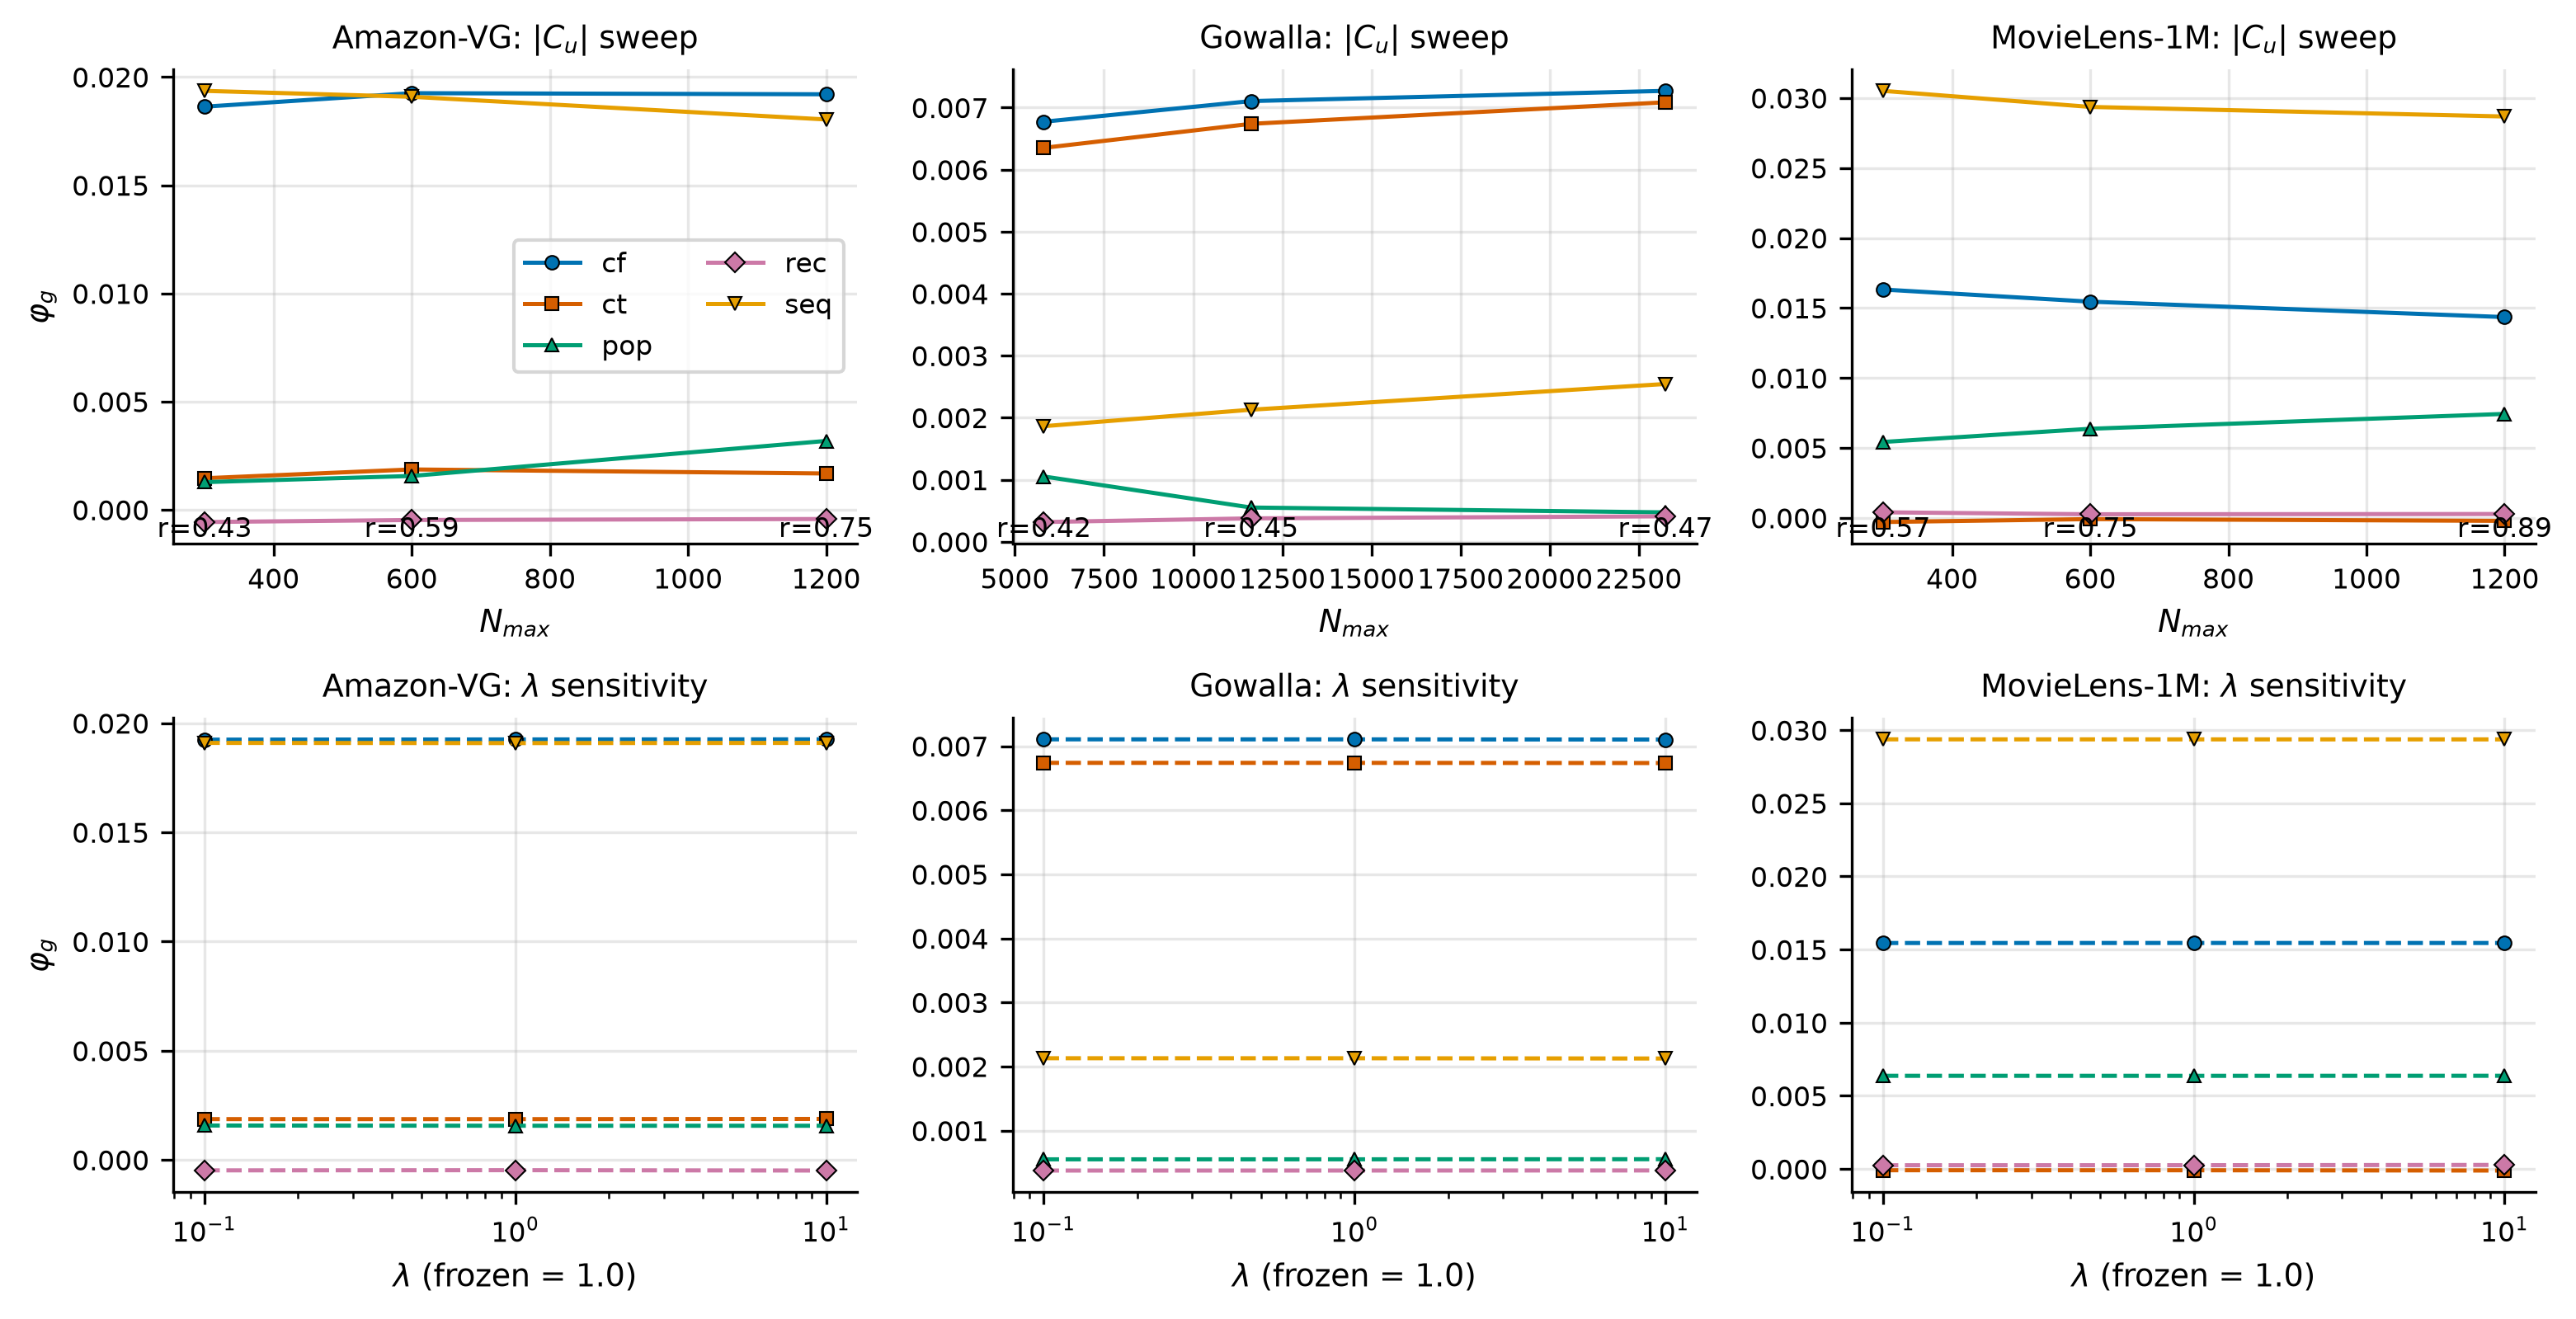
\includegraphics[width=\linewidth]{F7_robustness.png}
\caption{Robustness. Candidate recall is annotated per cell of the $|\Cu|$
sweep, because changing $|\Cu|$ moves the recall ceiling and hence the level of
$v$; without it the cells are not comparable. The $\lambda$ panel is
sensitivity only and is never used for selection.}
\end{figure}

\begin{table}[htbp]
\centering
\footnotesize
\caption{T8 -- Robustness matrix. CANDIDATE RECALL IS REPORTED PER CELL for the $|C_u|$ sweep: changing $|C_u|$ moves the recall ceiling and hence the level of $v$, so without it the cells are not comparable.}
\label{tab:T8_robustness}
\begin{tabular}{lllll}
\toprule
Dataset & Stress test & Candidate recall & Top source & $v(\mathcal{G})$ \\
\midrule
ml\_1m & $|C_u|$ = 300 & 0.566 & seq & 0.05231 \\
ml\_1m & $|C_u|$ = 600 & 0.748 & seq & 0.05253 \\
ml\_1m & $|C_u|$ = 1200 & 0.890 & seq & 0.04891 \\
ml\_1m & $\lambda$ = 0.1 & -- & seq & -- \\
ml\_1m & $\lambda$ = 1.0 & -- & seq & -- \\
ml\_1m & $\lambda$ = 10.0 & -- & seq & -- \\
ml\_1m & rescale: identity & -- & seq & -- \\
ml\_1m & rescale: log1p & -- & seq & -- \\
ml\_1m & rescale: rank & -- & seq & -- \\
\bottomrule
\end{tabular}
\end{table}


Shapley orderings are stable across candidate-set size and across an order of
magnitude of $\lambda$ either side of the frozen value. Rank and $\log 1p$
rescalings do shift attributions, as Remark~1 predicts: invariance is affine
only, and this is the empirical content of the remark rather than a defect.

\begin{table}[htbp]
\centering
\footnotesize
\caption{T4 -- Computational cost. The 'laptop CPU, seconds' claim applies to the Shapley computation (32-coalition sweep and downstream analysis); base-scorer training is a separate one-time cost.}
\label{tab:T4_cost}
\begin{tabular}{lllll}
\toprule
Dataset & Scorers (train once, s) & Candidates (s) & 32 coalitions (s) & Total (s) \\
\midrule
ml\_1m & 16.52 & 8.45 & 17.00 & 164.54 \\
\bottomrule
\end{tabular}
\end{table}


The 32-coalition sweep and all downstream analysis run in seconds of laptop CPU
time. We note this claim applies to the Shapley computation; base-scorer
training is a separate one-time cost.

%% ===================================================================
\section{Limitations}\label{sec:limitations}
%% ===================================================================

We separate what is established from what is not.

\paragraph{Analytic and data-independent.} The counterexample refuting
unconditional Property~\ref{prop:loo}; the $1/|\G|$ constant in
Lemma~\ref{lem:eps}; the bias argument against grand-coalition candidate pools;
the bias argument against per-coalition $\lambda$ tuning. These are
mathematical and do not depend on any corpus.

\paragraph{Pilot-only.} \emph{Every numeric result in
\S\ref{sec:results}--\S\ref{sec:negative}.} These come from a controlled
synthetic pilot with planted structure, built to validate the estimator and
exercise the pipeline end to end. They establish that the machinery is correct
and the analysis executable; they establish nothing about MovieLens-1M,
Amazon-Book, or LastFM-2K. In particular the negative result of
\S\ref{sec:negative} may well reverse on real corpora, where genuine behavioural
heterogeneity is plausible --- the planted structure was not designed to contain
it. Benchmark results are the immediate next step and the artefact runs them
with one command.

\paragraph{Two datasets miss the recall gate.} At the pre-registered
$N_{\max}$, LastFM-2K (0.504) and Amazon-Book (0.402) fall below the 0.60 floor.
Their attribution numbers are reported \emph{conditional on} that ceiling and
should not be read as absolute ranking quality.

\paragraph{The fitted game is non-monotone.} Consequently
Property~\ref{prop:loo} is not applicable as stated on this data, and
Lemma~\ref{lem:eps}(ii) requires restatement under bounded synergy.

\paragraph{Scope.} Five sources; the exact approach does not extend
indefinitely, and beyond roughly 20 players a hybrid exact-plus-sampled scheme
would be required. Attribution is within the fixed candidate set and carries no
causal interpretation.

%% ===================================================================
\section{Conclusion}
%% ===================================================================

We formulated hybrid-recommender source attribution as a five-player
cooperative game and computed exact Shapley values over all 32 coalitions,
avoiding the estimator variance that forces feature-level Shapley to sample. We
showed that a natural statement of the redundancy property is false without
monotonicity, gave the counterexample, and audited the hypothesis rather than
assuming it. On a controlled pilot, LOO and exact Shapley disagreed
qualitatively --- LOO judged three of five useful sources harmful --- which is
the practical case for the method. We also report, in full, that
segment-adaptive fusion produced no gain, and we traced the cause to an absence
of the segment heterogeneity such fusion presupposes.

Immediate future work is the benchmark evaluation on real corpora that the
artefact is built to run. Beyond that: privacy-bearing signals as players,
cascade hybrids, and causal extensions of source attribution.

%% ===================================================================
\section*{Declarations}
%% ===================================================================

\paragraph{Funding.} [To be completed.]

\paragraph{Competing interests.} The authors declare none.

\paragraph{Ethics approval.} Not applicable: no human-subjects data or
biological material. Public benchmarks are used under the licenses named in the
artefact.

\paragraph{Data availability.} Code, configuration, cached matrices, and every
artefact JSON backing the numbers above will be archived on Zenodo with a DOI
at publication. MovieLens-1M is used under the GroupLens research-use license;
LastFM-2K under HetRec 2011 / GroupLens non-commercial research terms;
Amazon-Book per the dataset host's academic-use conditions.

\paragraph{Author contributions (CRediT).} \textbf{M. Louhichi:}
conceptualisation, methodology, software, formal analysis, investigation,
writing --- original draft, visualisation. \textbf{R. Nesmaoui:} software,
validation, data curation, writing --- review \& editing.
\textbf{M. Lazaar:} supervision, methodology, resources, writing ---
review \& editing, funding acquisition.

\paragraph{Use of AI tools.} Large language models were used for code
scaffolding, editorial review of the manuscript, and consistency checking of
the specification. All mathematical claims were independently verified, and the
counterexample in \S\ref{sec:theory} is machine-checked in the artefact's test
suite. The authors take full responsibility for the content.

\paragraph{Reproducibility.}\label{sec:repro} Every number traces to a JSON
file in \texttt{artefacts/}; no value is transcribed by hand into a table.
Configuration is pre-registered and frozen. Two invariants are enforced in
continuous integration: the counterexample pinning the monotonicity hypothesis,
and the dataset density ordering on which the cross-corpus comparison rests.

\bibliographystyle{unsrtnat}
\bibliography{paper}

\appendix
\section{Derivations}
Full derivations of Properties~1--3 and Lemma~\ref{lem:eps}, including the
counterexample payoff tables in machine-checkable form, accompany the artefact.

\end{document}
